\chapter{基于GPU的实时磁共振指纹的字典生成和匹配}
\label{chap:snapMRF}
磁共振指纹(magnetic resonance fingerprinting, MRF)是定量MRI技术的新方法,可以在单次扫描中同时获得多个组织参数\cite{mrf,esr,bipin_mehta_magnetic_2019},因此MRF有着加速MR成像的潜力。MRF主要包括三个部分,分别为信号采集、字典生成和模式识别。其中信号采集的速度取决于MR自身扫描的速度,而字典生成和模式识别则取决于算法和硬件。因此一个快速开源的MRF重建程序可以增加MRF临床应用的可行性和准确率。

\section{MRF重建参数图的主要问题}
MRF重建参数图的一个重要过程是生成包含不同组织参数模拟信号的字典。MRF重建的准确性很大程度上取决于模拟信号的准确性。在MRF最早的文章中,Ma等\cite{mrf}使用了Bloch方程来模拟单个等色子在MR序列中的演化。模型假设指纹中的每个体素都由单一等色子构成,可以很好地模拟bSSFP序列的演化过程。但是当处理uSSFP序列时,Bloch模型必须将所有等色子考虑进去。这是因为在uSSFP中,由于非平衡梯度场的存在,指纹中的每个体素都是多个等色子的平均。因此Bloch方程在处理uSSFP时的效率不高。

扩展相图是用来模拟MR成像的另一个模型,曾经被用在\cite{jiang}中。有关EPG的详细信息请参考第\ref{sec:epg}小节。EPG利用Fourier变换将自旋系统描述为多个离散的配置状态。相对于Bloch方程,EPG可以提供更准确的信号演化,尤其是当自旋系统受到非均匀磁场的影响时,比如在uSSFP中常用的破坏梯度场。但是EPG模型的计算很耗时,因为为了确保结果的准确性,对于每个模拟信号我们都需要追踪100个甚至更多的配置状态。这在程序中体现为一个维度很高的矩阵,对计算速度和计算机存储都是很大的负担。如果只在CPU上运行,在我们自己的硬件上生成一个和Ma等\cite{mrf}使用的同样大小的字典需要几个小时。所以增加模型准确性的代价是巨大的。

除了字典的生成,模式识别也非常耗时。模式识别是将采集到的指纹数据和字典进行匹配,Ma等\cite{mrf}使用了模板匹配的方法来进行参数图的重建。记$X=\{x_n\in \mathbb{C}^L\}, n=1,...,N$为采集到的指纹数据,$\mathcal{D}=\{d_k\in \mathbb{C}^L\},k=1,...,K$为生成的字典。那么模板匹配即为从从字典$\mathcal{D}$中选取和$x_n$内积最大的元素:
	\begin{equation}
	\hat{k}_n = \argmax_k \left|\left\langle \mathbf{d}_k,\mathbf{x}_n \right\rangle \right|.
	\end{equation}
并且质子密度也可以同时计算:
	\begin{equation}
	\hat{\rho}_n=\left|\langle \mathbf{d}_{\hat{k}_n},\mathbf{x}_n \rangle\right|.
	\end{equation}
不难看出,模板匹配的运行时间与字典大小$K$,时间点的个数$L$以及指纹数据中体素的个数有关,计算复杂度为$O(NL^2K)$。当字典很大,指纹数据很多的时候,重建参数图所消耗的时间是许多快速成像方法无法容忍的。比如,Ma等在\cite{mrf}中使用生成了一个大小为566,783的字典,其中时间点为1,000,并将其和128$\times$128个体素进行匹配。在他们自己的硬件上,使用MATLAB程序运行,字典生成花费了399 s,而匹配花费了大约3分钟。

在第\ref{sec:mrf}节中,我么回顾了MRF加速的常用方法。其中一大类是基于降维的方法,通过降低字典或者数据的维度,从而达到加速计算的目的。常用的策略是压缩字典在时间方向的维度,比如MaGiney\cite{svdmrf}利用奇异值分解来压缩字典在时间方向的维度,使得模板匹配得到了3.4--4.8倍的加速。但是大矩阵奇异值的计算本身计算消耗就很多大,而且在依然需要先生成一个字典。Cauley等\cite{groupingmrf}提出了分组的思想来处理字典,先将字典中的元素聚类,再用主成分分析来压缩字典在时间和参数方向的维度。这两种方法均没有加速字典生成,而且得到的结果只是模板匹配的近似,因而存在误差。

另一种加速方法是使用神经网络来学习重建参数图\cite{cohen2018mr},使用神经网络对参数图直接推断比在整个字典上进行模板匹配快得多。但是基于学习的方法有一个缺陷就是,学习和训练的效果很大程度上取决于样本的好坏,即网络的训练需要生成字典和其匹配的结果。如果成像序列发生了轻微的变化,比如偏转角、$T_\mathrm{R}$或者$T_\mathrm{E}$发生了变化,我们必须重新生成字典并且重新训练网络。理想的解决方式是每当采样序列发生变化时,都能够快速甚至即时的生成新字典。如果能将字典生成和匹配的程序适当地并行运行,这样的解决的方式是可以达到的。

\section{基于GPU的MRF重建}
目前的方法均从模型和算法的角度来提高MRF重建参数图的速度,而另一个思路是通过合理利用计算机硬件,编写并优化程序来加速MRF重建。Malik等\cite{malik_extended_2018}发布了一款基于MATLAB语言的程序EPG-X,可以为不同的MR序列进行建模。但是由于他们的程序运行在CPU上,速度很慢,尤其是字典生成的速度。同时,EPG-X不能够处理变化回波时间(variable $T_\mathrm{E}$)或者变化重复时间(variable $T_\mathrm{R}$)的序列,而这两种序列在MRF中经常遇到。此外,EPG-X也不能处理$B_1^+$效应,我们可以从后面的数值实验中看到,考虑$B_1^+$可以提高参数图的准确性。Cloos\cite{cline2017air}等编写了一款基于C++语言的程序PnP-MRF,可以模拟整个MRF重建的过程。PnP-MRF生成字典的速度虽然较快,但模板匹配的速度很慢。而且PnP-MRF只使用了Bloch方程来生成字典,不能实现EPG模型,并且和EPG-X一样,PnP-MRF不能够实现$B_1^+$校正。

最近几年,图形处理单元(graphic processing units,GPU)逐渐成为加速科学计算的主流方法,并在医学成像领域有着广泛的应用,详细的综述请参考文献\cite{gpu}。GPU中集成了大规模并行计算单元,在允许使用复杂模型的同时,保持合理的执行时间。GPU有以下两个主要特点:第一,与传统CPU芯片不同,GPU中用于浮点运算的空间要远远多于指令分配,因此具有强大的科学计算潜力;第二,可编程的特性,即用户可以通过应用程序接口直接在GPU上进行编程,体现了很好的交互能力。这两个特点奠定了GPU并行计算的基石。目前应用最广泛的应用程序接口是Nvidia公司的CUDA框架,其提供的编程能力在显著地发展,程序的复杂度也在慢慢地减少。基于CUDA框架的GPU编程需要注意以下三点。第一,需要对GPU硬件有足够的了解,这样才能充分发挥GPU的潜力。第二,合理地为程序中的变量分配显存,使得线程尽量可以访问连续的显存空间,这样可以大大减少线程访问显存的时间。第三,避免条件竞争的发生,即避免不同线程同时写入同一显存位置,从而造成不确定的结果。简而言之,GPU编程是一个根据使用的硬件不断调试和优化的过程,其通常能够使得程序运算速度提高10--100倍。

目前,GPU并行计算已经被广泛地应用于医学成像领域,如CT\cite{biguri2016tigre,palenstijn2011performance}、MRI\cite{Knoll,Sorensen,tron,Eklund2014BROCCOLI,Xanthis2014MRISIMUL}、US\cite{Jung2013GPU,Yakang2010Real}、PET\cite{Garcia2016Accelerated,Cui2013Distributed}等。但是据我们所知,目前没有程序在CUDA的框架下,利用GPU来实现MRF的字典生成和模板匹配。另外,也有一些文献中也表明了对缺少科学研究的可重复性的担忧\cite{vasilevsy_repro_2013,osc_repro_2015,collins_repro_2014,begley_repro_2015}。针对以上问题,我们开发了一款基于GPU的开源MRF重建程序snapMRF,用于并行计算字典生成和模板匹配。snapMRF将字典生成和模板匹配全部放在GPU上并行计算,并且给出了一系列单元测试来保证程序的可靠性和准确性。snapMRF既可以用Bloch方程也可以用EPG模型来进行字典生成,保证了程序的普适性。

\section{snapMRF程序设计与单元测试}
\subsection{snapMRF程序流程与难点}
snapMRF实现MRF重建参数图的过程一共可以分为5个步骤,其中前两个步骤为指纹数据与成像参数的输入,后面的两个步骤为字典的生成与匹配,最后一个步骤为结果的输出,如图\ref{fig:snapmrf}所示。这样的设计框架由GPU计算的原理所决定的。一般来说,利用GPU进行并行计算需要首先将数据从主机(host)拷贝到设备(device)上,在设备上进行计算之后,再将处理之后的数据从设备拷贝回主机上进行存储或其他处理。这样做是为了尽可能避免数据在主机和设备之间进行多次拷贝,减少时间消耗。注意下面变量前面的 * 表示C语言中的向量指针,其中主机向量指针以字母\texttt{h}开头,设备向量指针以字母\texttt{d}开头。
\begin{figure}
\centering
 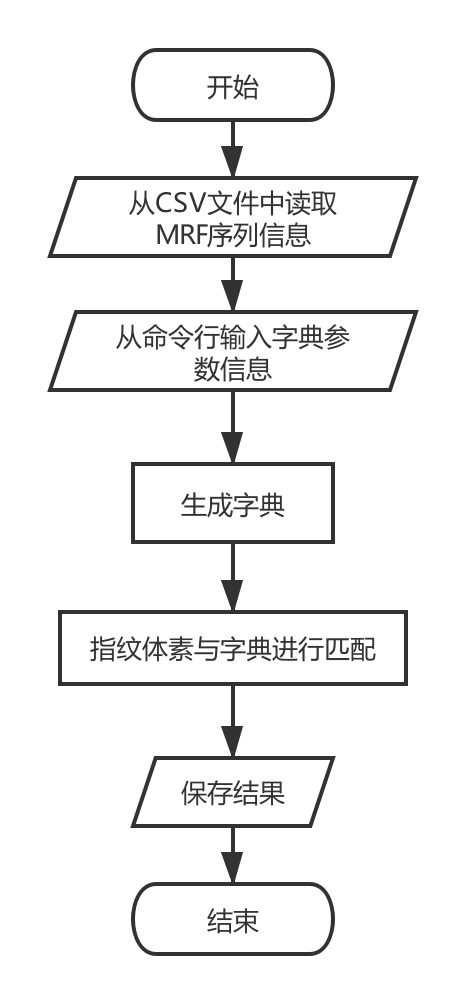
\includegraphics[width=1\textwidth]{img/snapmrf/snapMRF.png}
\caption{snapMRF流程图。}
\label{fig:snapmrf}
\end{figure}

\begin{itemize}
\item \textbf{从CSV文件中读取MR序列的成像参数},将其存储在主机向量\texttt{*h\_mrf},并拷贝到设备向量\texttt{*d\_mrf}中。这个CSV文件中包含了MR序列的信息,即偏转角$\alpha$,相位角$\Phi$,回波时间$T_\mathrm{E}$和重复时间$T_\mathrm{R}$。时间点的个数储存在变量\texttt{nreps}中。

\item \textbf{从命令行读取字典的配置信息($T_1$, $T_2$, $B_0$, $B_1^+$).}使用函数\texttt{parse\_length()}解析命令行,并使用函数\texttt{parse\_params()}将其分别储存在主机向量\texttt{*h\_t1}, \texttt{*h\_t2},\texttt{*h\_b0}和\texttt{*h\_b1}中。为了之后处理方便,这四个主机向量被函数\texttt{trans\_params()}合并成一个向量,并拷贝到设备向量\texttt{*d\_params}。在\texttt{*d\_params}中,配置信息的存储顺序是$T_1$优先的,即$T_1$的指标变化最快,然后是$T_2$,然后是$B_0$,$B_1^+$的指标变化最慢。配置信息的个数分别存放在变量\texttt{l\_t1}, \texttt{l\_t2}, \texttt{l\_b0}和\texttt{l\_b1}中。字典中元素的个数通过函数\texttt{compute\_natoms()}计算得到,存储在变量\texttt{natoms}中。由于在实际情况中,$T_1$的值一般远大于$T_2$的值,所以$T_1 \le T_2$的情况被移除了。

\item \textbf{生成字典},使用的函数为\texttt{MRF\_dict()},并将结果储存在设备向量\texttt{*d\_atoms}中。这是程序设计中最有难度的一个步骤。对于每个$B_1^+$和每个时间点,设备函数关于字典中元素的指标是并行计算的。也就是说,字典中所有元素的信号演化是并行计算的,即我们先计算所有元素在第一个时间点的信号大小,更新每个元素的状态矩阵\texttt{*d\_w},之后计算下一个时间点的信号大小,直至所有时间点都计算结束。其中状态矩阵\texttt{*d\_w}包含了字典中所有元素的状态矩阵,其维度为$(3\times \texttt{nstates})\times \texttt{natoms}$,其中每个元素的状态矩阵的维度为$3\times \texttt{nstates}$。由于状态矩阵的维度通常很大,这会给显存带来很大的负担,并且造成计算资源的浪费。因此,字典生成结束后,我们需要将\texttt{*d\_w}释放。字典中元素所包含的参数信息存储在\texttt{*d\_params}中,顺序与字典\texttt{*d\_atoms}相同。

\item \textbf{将指纹体素与字典匹配}。从RawArray \cite{RawArray}文件中读取采集好的指纹数据,存储在向量\texttt{*d\_img}中。函数\texttt{MRF\_match()}分两步计算参数图。第一步,对于每个包含不同$B_1^+$的子字典,计算指纹数据在子字典下的参数图,并将其储存在\texttt{*d\_MAPS}中。当字典过大时,GPU的显存可能有限。为了最大程度地利用GPU的显存,我们首先计算程序运行到此处时GPU所剩显存,并用函数\texttt{compute\_nsplits()}根据所剩显存将指纹数据分为大小相等的组,在每个小组上进行匹配。函数\\ \texttt{MRF\_minimatch()}用来计算每个小组的指纹数据的参数图。同时为了优化匹配速度,我们将指纹数据看做一个矩阵,则指纹与字典的内积则可以由指纹与字典的共轭转置相乘得到。这样做的目的是为了使用高度优化的cuBLAS软件库中矩阵相乘的函数。然后利用函数\texttt{generate\_maps()}从内积矩阵中生成参数图。第二步,使用\texttt{merge\_maps()}将不同$B_1^+$生成的参数图融合起来,生成最终的参数图。这个设备函数关于体素是并行计算的。对于每个体素,由于在第一步中产生了\texttt{l\_b1}组参数,选择与校正$B_1^+$最接近的那个$B_1^+$的值,并将其相对应的$T_1$, $T_2$和$B_0$作为最后的参数,最接近校正值的$B_1^+$也被保存了下来。最后的参数图在\texttt{*d\_maps}中,以$T_1$, $T_2$, $B_0$, $B_1^+$和质子密度的顺序存储。

\item \textbf{保存结果}。将字典元素\texttt{*d\_atoms}和参数图\texttt{*d\_maps}从GPU拷贝回CPU,并存储成为RawArray格式。释放内存。

\end{itemize}

从以上步骤可以看出,snapMRF程序设计中的难点和创新主要有以下几点。第一,确定多维向量指针在显存中的储存结构,其目的是保证线程可以连续地访问显存空间。我们需要确定一个指标变化的优先级,即多维向量指针指标变化的快慢。对于包含时间维度的向量指针,如\texttt{*d\_atoms}、\texttt{*d\_mrf}、\texttt{*d\_img}等,我们选取时间维度优先,即时间方向的指标变化最快。对于包含参数维度的向量指针,如\texttt{*d\_maps}、\texttt{*d\_params}等,我们选取参数维度优先,即参数方向的指标变化最快。第二,计算多维向量在显存中对应的一维指标。字典、指纹等数据虽然为多维数据,但其在显存中的储存和访问只能是一维线性的。因此,多维数据的指标和其在显存中的一维指标需要一一对应起来。这一点至关重要,因为一旦指标计算错误,最后的结果会变得无法预测且这种错误很难被发现。第三,管理显存。为了使得GPU的显存得到充分的利用,我们需要时刻注意剩余显存的大小,在不超过显存上限的前提下,最大限度的利用显存。snapMRF中,在进行字典匹配之前,我们首先释放了\texttt{*d\_w}的显存,并且计算了此时剩余显存的大小,然后根据剩余显存的大小来为后面的数据分配显存。第四,snapMRF中主机与设备之间的数据拷贝只发生两次,分别为将MR成像序列和指纹数据从CPU拷贝到GPU和将计算结果从GPU拷贝到CPU,其余所有计算均在GPU上进行,最大限度地减少了数据拷贝的时间开销。

\subsection{snapMRF核函数的功能}
在Nvidia的计算框架CUDA中,将在GPU上并行计算的特殊函数称为核函数(kernel),将该函数运行的一个实例称为一个线程(thread)。因此GPU并行计算编程的一个原则是将复杂的算法分解,使得算法的每一小步都可以在GPU上通过核函数并行运行。我们下边简单介绍snapMRF中核函数的主要功能,如表\ref{tab:kernel}所示。

\begin{itemize}
	\item \texttt{init\_rf\_pulse()} 默认初始化磁化向量大小为状态$[0,0,1]^T$。如果使用的序列为uSSFP,对初始磁化进行反转衰减(inversion decay),衰减时间为\texttt{TI} ms。核的输入为字典大小\texttt{natoms}和状态的个数\texttt{nstates},输出为状态矩阵\texttt{*d\_w}。 
	
	\item \texttt{fill\_transition\_matrix()}根据偏转角和相位角计算转移矩阵\texttt{*d\_T\_m}中的每一个元素,其中偏转角和相位角储存在向量\texttt{*d\_mrf}中。转移矩阵\texttt{*d\_T\_m}对应EPG算法中的$T$算子,它的作用是模拟射频场对磁化的影响。
	
	\item \texttt{apply\_rf\_pulse()}将转移矩阵\texttt{*d\_T\_m}作用于状态矩阵\texttt{*d\_w}上。这里单精度复值矩阵乘法使用CUDA自带的cuBLAS函数库中的函数\texttt{cublasCgemm()}实现。
	
	\item \texttt{shift\_phase()}磁化的水平分量相位平移作用在状态矩阵\texttt{*d\_w}上。这个核只有在bSSFP序列中用到。
	
	\item \texttt{save\_atom()}从状态矩阵\texttt{*d\_w}中读取最近的回波强度,并储存在字典\texttt{*d\_atoms}中。输入为序列中时间点的个数\texttt{nreps}和当前回波所在的时间点\texttt{index}。
	
	\item \texttt{decay\_signal()}将$T_1$和$T_2$衰减作用在状态矩阵\texttt{*d\_w}中并把结果保存在状态矩阵中。这里衰减的时间有四种不同的选择,分别为:$T_\mathrm{E}$ (\texttt{type=1}),$T_\mathrm{R}-T_\mathrm{E}$ (\texttt{type=2}),$T_\mathrm{E}/2$ (\texttt{type=3})和$T_\mathrm{R}$ (\texttt{type=4})。$T_\mathrm{E}$和$T_\mathrm{R}$存储在向量\texttt{*d\_mrf}中,而$T_1$和$T_2$存储在向量{*d\_params}。这个核相当于EPG模型中的$E$算子。
	
	\item \texttt{dephase\_gradients()}将失相效果作用于状态矩阵\texttt{*d\_w}上,并将结果保存回状态矩阵。这个核相当于EPG模型中的$H$算子。
\end{itemize}

\begin{table}
\centering
\caption{snapMRF中的核函数}
\begin{center}
\begin{tabular}{|l|l|l|l|}
\hline
\hline
核函数 & 输入 & 输出 & 算子\\
\hline
\texttt{init\_rf\_pulse()} & \texttt{natoms}, \texttt{nstates} & \texttt{*d\_w} & - \\
\hline
\texttt{fill\_transition\_matrix()} & \texttt{*d\_mrf} & \texttt{*d\_T\_m} & $T$ \\
\hline
\texttt{apply\_rf\_pulse()} & \texttt{*d\_w}, \texttt{*d\_T\_m} & \texttt{*d\_w} & - \\
\hline
\texttt{shift\_phase()} & \texttt{*d\_w} & \texttt{*d\_w} & - \\
\hline
\texttt{save\_atom()} & \texttt{*d\_w}, \texttt{nreps}, \texttt{index} & \texttt{*d\_atoms} & - \\
\hline
\texttt{decay\_signal()} & \texttt{*d\_w}, \texttt{*d\_params} & \texttt{*d\_w}  & $E$ \\
\hline
\texttt{dephase\_gradients()} & \texttt{*d\_w} & \texttt{*d\_w} & $H$ \\
\hline
\end{tabular}
\end{center}
\label{tab:kernel}
\end{table}

\subsection{单元测试}
单元测试是简单的情形的测试,目的是为验证和确保程序的正确性。单元测试的正常结果是全部通过。如果有一个或者多个单元测试失败,那么意味着程序或者算法有错误。snapMRF中给出了8组单元测试,每组单元测试对应一个简单序列的字典生成或者模板匹配,并与其相对应的解析解进行比较。所有的单元测试都包含在源文件\texttt{test.cu}中。Table \ref{tab:unittest}显示了不同序列所用到的参数。单元测试共使用了6个不同的序列,每个序列都有不同的参数。$[a,b]$意思是参数是在区间$a$与$b$中随机选择。为了简化计算,对于所有的序列,$B_0=0$并且$B_1=1$。序列的详细信息请参考文献\cite{weigel}和\cite{web}。

\begin{table}
\centering
\caption{单元测试中使用的参数}
\begin{center}
\begin{tabular}{|l|l|l|l|l|l|l|}
\hline
\hline
序列类型 & $\alpha$ (deg) & $\Phi$ (deg) & $T_1$ (ms) & $T_2$ (ms) & $T_\mathrm{E}$ (ms) & $T_\mathrm{R}$ (ms)\\
\hline
SE & $\frac{\pi}{2}\rightarrow\pi$ & $\frac{\pi}{2}\rightarrow0$ & 600 & 100 & 25 & 1000\\
\hline
SR & $\frac{\pi}{3}\rightarrow\cdots$ & $\frac{\pi}{2}\rightarrow \cdots$ & 600 & 100 & 1 & 500\\
\hline
FSE & $\frac{\pi}{2}\rightarrow\frac{2\pi}{3}\rightarrow\cdots$ & $\frac{\pi}{2}\rightarrow0\rightarrow\cdots$ & - & - & 0 & 0\\
\hline
FSE+relax & $\frac{\pi}{2}\rightarrow\pi\rightarrow\cdots$ & $\frac{\pi}{2}\rightarrow0\rightarrow\cdots$ & 600 & 100 & 25 & 50\\
\hline
FISP & $\frac{\pi}{6}\rightarrow\cdots$ & $0\rightarrow\cdots$ & 1000 & 100 & 5 & 10\\
\hline
SSFP & [0,$\pi$/3] & $0\rightarrow\cdots$  & 100,200 & 20,40 & [3.5,7.5] & 16\\
\hline
\end{tabular}
\end{center}
\label{tab:unittest}
\end{table}

%\subsection{自旋回波}
第一个单元测试的序列是一个简单的自旋回波,由一个90$^{\circ}$(偏转角$\alpha = \pi/2$,相位角$\Phi = \pi/2$)和一个180$^{\circ}$(偏转角$\alpha = \pi$,相位角$\Phi = 0$)射频脉冲构成。其中$T_1 = 600$ ms,$T_2 = 100$ ms,$T_\mathrm{E} = 25$ ms,$T_\mathrm{R} = 1000$ ms。通过简单计算可以得知,这个回波产生的信号为$(e^{-T_\mathrm{E}/T_2})^2 =[\exp(25/100)]^2=0.6065$。snapMRF中相应的函数为\texttt{epg\_se()}。注意这里$T_\mathrm{E}$的含义与传统自旋回波不同。在传统自选回波中,$T_\mathrm{E}$是指90$^{\circ}$射频脉冲到读取回波的时间。但是在snapMRF中,由于程序是由稳态序列优化,这里的回波时间是指180$^{\circ}$射频脉冲到读取回波的时间。如果想把这里的$T_\mathrm{E}$转换为传统的自旋回波$T_\mathrm{E}$,只需要将其除以2。同样的情况也是用与快速自旋回波。

%\subsection{饱和恢复序列}
第二个单元测试是饱和恢复序列(saturation recovery),由60$^{\circ}$相隔时间相同(偏转角$\alpha = \pi/3$,相位角$\Phi = \pi/2$)的射频脉冲构成。这里其中$T_1 = 600$ ms,$T_2 = 100$ ms,$T_\mathrm{E} = 1$ ms,$T_\mathrm{R} = 500$ ms。经计算得到解析解为$[$0.857, 0.674, 0.631, 0.622, 0.620, 0.620, 0.620, 0.620, 0.620, 0.620$]$。snapMRF中相应的函数为\texttt{epg\_sr()}。可以看出,在经历了几个脉冲序列之后,回波强度达到了稳态。

%\subsection{无驰豫快速自旋回波}
第三个单元测试是无驰豫快速自旋回波序列(fast spin echo),由一个90$^{\circ}$(偏转角$\alpha = \pi/2$,相位角$\Phi = \pi/2$)和一系列120$^{\circ}$(偏转角$\alpha = 2\pi/3$,相位角$\Phi = 0$)射频脉冲构成。既然驰豫被忽略,在理论上$T_1$和$T_2$的值应为正无穷。因此,在程序中$T_1$和$T_2$并未被真正用到。我们只计算了三个回波,最后回波的强度为$[$0.750, 0.938, 0.844$]$。snapMRF中相应的函数为\texttt{epg\_tse()}。

%\subsection{有驰豫快速自旋回波}
第四个单元测试是有驰豫快速自旋回波序列,由一个90$^{\circ}$(偏转角$\alpha = \pi/2$,相位角$\Phi = \pi/2$)和8个180$^{\circ}$(偏转角$\alpha = \pi$,相位角$\Phi = 0$)射频脉冲构成。这里$T_1 = 600$ ms,$T_2 = 100$ ms,$T_\mathrm{E} = 25$ ms,$T_\mathrm{R} = 50$ ms。最后的回波为$[$0.607, 0.368, 0.223, 0.235, 0.082, 0.0500, 0.0302, 0.0183, 0.0111, 0.0068$]$。snapMRF中相应的函数为\texttt{epg\_tse()}。

%\subsection{快速梯度回波}
第五个单元测试是$F_0$-type SSFP序列(也成为FISP),由一系列30$^{\circ}$(偏转角$\alpha = \pi/6$,相位角$\Phi = 0$)射频脉冲构成。这里$T_1 = 1000$ ms,$T_2 = 100$ ms,$T_\mathrm{E} = 5$ ms,$T_\mathrm{R} = 10$ ms。最后的回波为$[-0.4756i, -0.4125i, -0.3358i]$。snapMRF中相应的函数为\texttt{epg\_fisp()}。

%\subsection{Bloch方程}
第六个单元测试是翻转恢复平衡自由进动(IR-bSSFP)序列,使用Bloch方程来生成模拟信号。我们生成了一个含有4个元素的字典,字典中的每个元素有4个时间点。snapMRF中相应的函数为\texttt{roa\_ssfp()}。

%\subsection{EPG模型}
第七个单元测试是翻转恢复平衡自由进动(IR-bSSFP)序列,使用EPG模型来生成模拟信号。我们生成了一个含有4个元素的字典,字典中的每个元素有4个时间点。snapMRF中相应的函数为\texttt{epg\_ssfp()}。

%\subsection{字典自匹配}
第八个单元测试是使用EPG生成的字典来进行自我匹配。我们从字典中随机选择10个体素作为指纹数据,并将其和字典进行匹配。对匹配的元素的验证确保了参数的正确性。snapMRF中相应的函数为\texttt{MRF\_match()}。

\section{数值实验数据与评价方法}
我们进行了三组数值实验,用于比较snapMRF与其他MRF开源程序,如EPG-X和PnP-MRF。数值实验所使用的数据以及评价方法如下。

\subsection{程序运行时间}
为了比较程序的运行时间,我们使用32通道的头部线圈对MRI系统体模 \cite{keenan_comparison_2016}(HPD, Boulder, Colorado) 在3.0 T(Philips Ingenia, Philips Healthcare, The Netherlands)进行冠状成像。体模在单个切片上成像,通过一系列不同MnCl$_2$浓度的对比度球得到不同的$T_1$和$T_2$值。体模的温度为20$^{\circ}$。k-space数据使用32倍均匀螺旋下采样获得\cite{pipe_spiral_2014}。图像的视野大小,平面内分辨率、平面外分辨率和螺旋采集时间分别为240 mm $\times$ 240 mm,1 mm $\times$ 1 mm,10 mm和4.9 ms。原始MRF数据使用BART\cite{bart}进行网格化和线圈组合重建,并且使用BART中的eSPIRIT估计线圈灵敏度图。样本密度使用\cite{zwart_sdc_2012}校正。重建后指纹数据的维度为$1000 \times 240 \times 240$。

体模数据所使用的MRF序列改变自将uSSFP用于MRF的第一篇文章\cite{jiang}。在这个序列中,绝热反转时间为40 ms,射频场为sinc-gauss型脉冲信号,并将时间带宽乘以10以最小化切片轮廓中$B_1^+$的异质性。重复时间$T_\mathrm{R}$和偏转角$\alpha$是变化的,其中$T_\mathrm{R}\in [16,18.7]$,$\alpha \in [0,60]$。回波时间$T_\mathrm{E}$固定在4.65 ms,总的扫描时间为17.5 s。

为了比较程序的运行时间,$T_1$的值设置为100 ms到3000 ms之间,$T_2$的值设置为20 ms到2000 ms之间。为了研究运行时间与字典大小的关系,我们选择了10组不同数目组合的$T_1$和$T_2$,共形成10个大小不同的字典。我们将snapMRF的运行时间与EPG-X\cite{malik_extended_2018}和PnP-MRF\cite{cloos2016multiparametric}比较,并画出运行时间随字典大小变化曲线。

\subsection{体模数据参数精度}
为了评估参数精度,我们比较了snapMRF与EPG-X生成$T_1$和$T_2$参数图的精度。在这组数值实验中,我们依然使用上一组数值试验中使用的体模数据。但是由于EPG-X只能处理固定$T_\mathrm{R}$的序列,我们使用固定$T_\mathrm{R}$的MRF序列对同样的体模数据进行成像。具体来说,$T_\mathrm{R}$固定在16 ms,其他参数均与上一组实验相同。原始MRF数据的重建也与上一组实验相同,最终重建后指纹的数据为$1500 \times 240 \times 240$。

为了对比snapMRF与EPG-X,我们首先比较二者在固定$T_\mathrm{R}$序列上重建参数图的精度。其次,我们比较snapMRF在固定$T_\mathrm{R}$和变化$T_\mathrm{R}$序列上表现的差异。最后我们研究$B_1^+$校正对参数图精度的影响。在所有比较中,我们均将字典大小选为100,000左右。不含$B_1^+$校正时,$T_1$的值从50 ms 到2500 ms,增量为5 ms,$T_2$的值从5 ms 到600 ms,增量为2.5 ms,最终字典大小为105,028。当考虑$B_1^+$校正时,$T_1$的值从50 ms 到2500 ms,增量为5 ms,$T_2$的值从5 ms 到600 ms,增量为2.5 ms,$B_1^+$的值从0.8到1.2,增量为0.1,最终字典的大小为105,655。参数图的精度使用相对误差来度量:
\begin{equation}
	\mathrm{err} = \frac{\|T_\mathrm{m}-T_\mathrm{gt}\|_2}{\|T_\mathrm{gt}\|_2}\times 100\%,
\end{equation}
其中$T_\mathrm{m}$是由snapMRF或者EPG-X生成的参数图,$T_\mathrm{gt}$是真实值。

\subsection{活体人脑数据}
为了评估图像质量,在评估委员会同意以后,我们在一位志愿者知情的情况下,使用32通道头部线圈在3.0 T(Philips Ingenia, Philips Healthcare, The Netherlands) 对其大脑横向切片成像。与体模数据相同,k-space数据使用32倍均匀螺旋下采样获得\cite{pipe_spiral_2014}。图像的视野大小,平面内分辨率、平面外分辨率和螺旋采集时间分别为240 mm $\times$ 240 mm,1 mm $\times$ 1 mm,5 mm和5.1 ms。原始MRF的重建算法和MRF的序列与体模数据均相同,最终形成指纹数据的维度为$1000 \times 240 \times 240$。

在本组数值实验中,我们从视觉上比较snapMRF与EPG-X生成参数图的好坏。与体模数据类似,我们也比较四种情形重建的参数图,即固定$T_\mathrm{R}$ EPG-X,固定$T_\mathrm{R}$ snapMRF,变化$T_\mathrm{R}$ snapMRF,变化$T_\mathrm{R}$ snapMRF加$B_1^+$校正。在所有比较中,我们均将字典大小选为100,000左右。不含$B_1^+$校正时,$T_1$的值从100 ms 到4000 ms,增量为10 ms,$T_2$的值从20 ms 到2000 ms,增量为5.5 ms,最终字典大小为108,056。当考虑$B_1^+$校正时,$T_1$的值从100 ms 到4000 ms,增量为20 ms,$T_2$的值从20 ms 到2000 ms,增量为14.5 ms,$B_1^+$的值从0.8到1.2,增量为0.1,最终字典的大小为102,830。

所有程序均在dual 10-core Intel Xeon E5-2630 2.20 GHz的CPU, 256 GB内存和Nvidia TITAN V的GPU的工作站上运行。snapMRF详细程序请参考网址\url{https://github.com/chixindebaoyu/snapMRF},版本为\texttt{v0.0.1}。

\section{数值实验结果}
\subsection{程序运行时间}
图\ref{fig:time}展示了snapMRF和EPG-X(上)与PnP-MRF(下)字典生成与模板匹配的运行时间的比较。注意图像中的曲线为对数尺度下的曲线。从图像中可以看出,所有时间曲线如设想一样随着字典大小呈线性变化。整体来看,snapMRF的运行速度是EPG-X与PnP-MRF的$10$--$100 \times$。具体来说,与EGP-X相比,snapMRF在字典生成方面(上,实线)的速度提高了60--1700$\times$,在模板匹配(上,虚线)上速度提高了2--20$\times$。与PnP-MRF相比,snapMRF在字典生成方面(下,实线)的速度提高了2--100$\times$,在模板匹配(下,虚线)上速度提高了60--500$\times$。因此,snapMRF在整体上字典生成的速度提高了10--1000$\times$,而模板匹配的速度提高了10--100$\times$。注意当字典比较大时,snapMRF的速度比其他两个程序快得多。

\begin{figure}
\centering
\begin{subfigure}
 \centering
 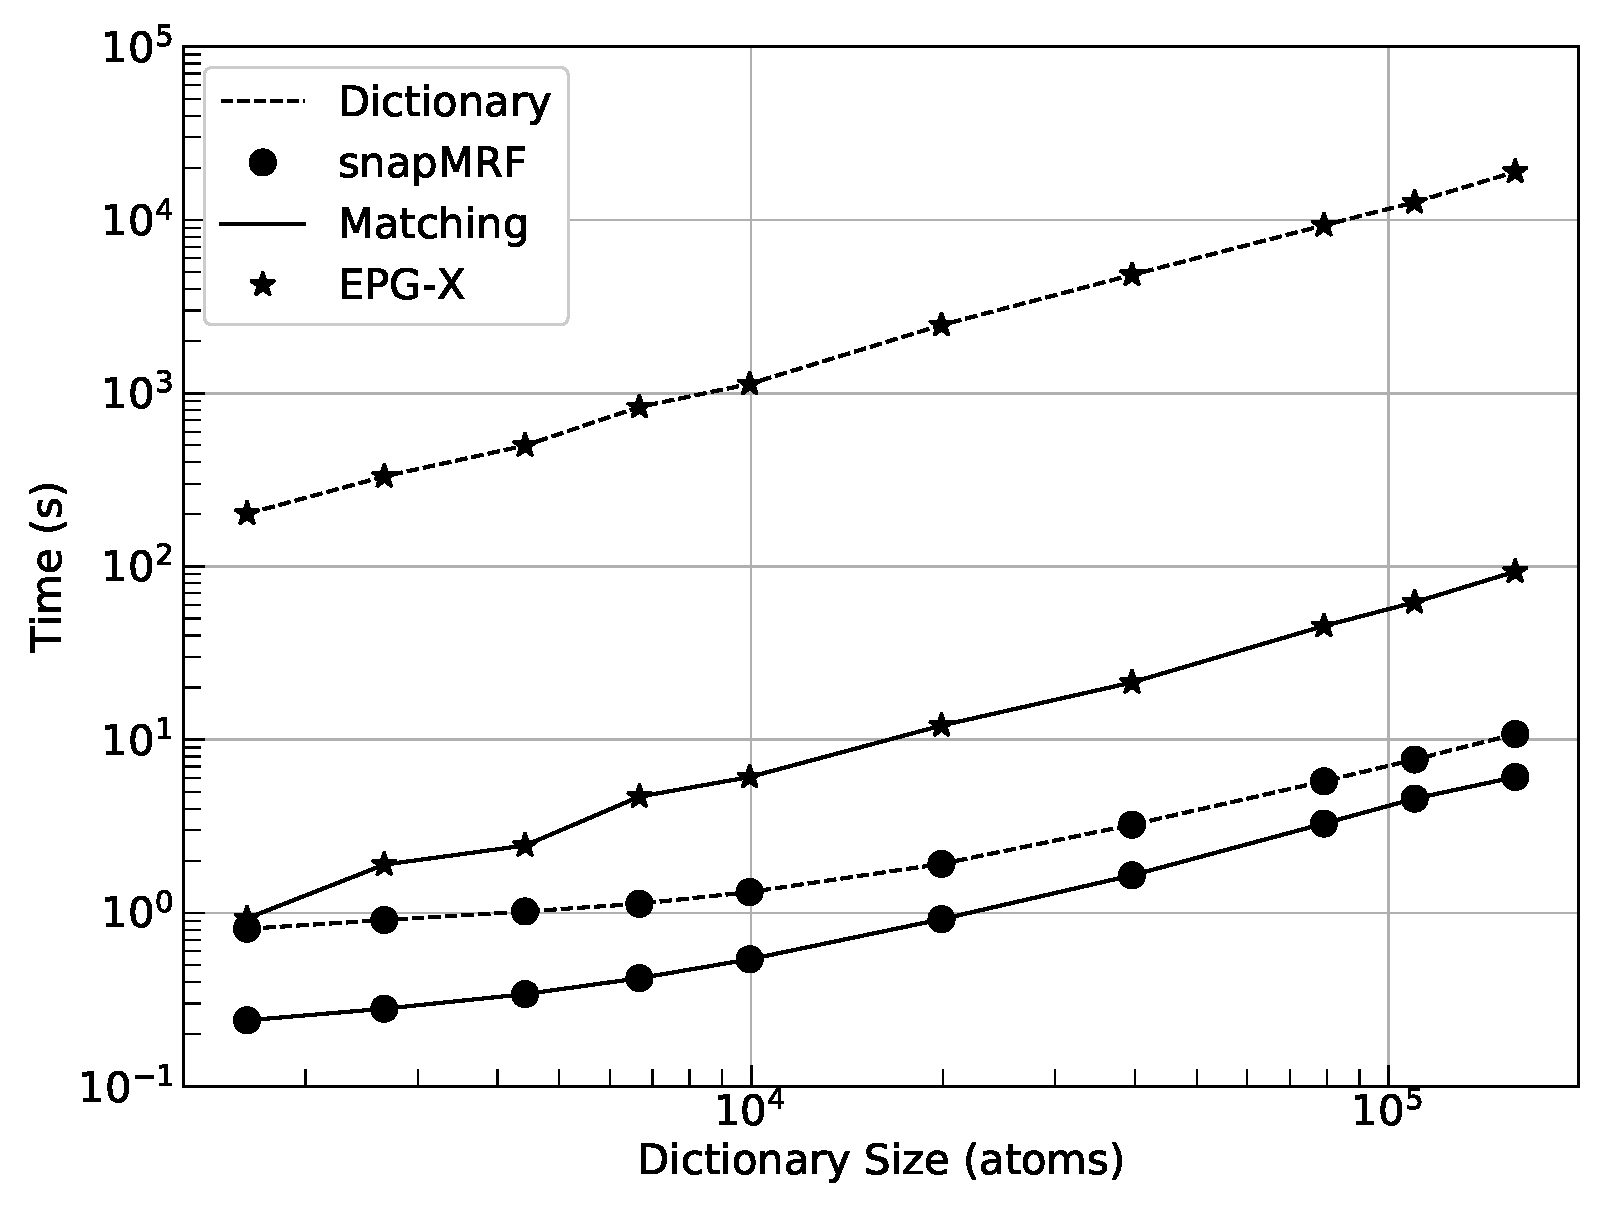
\includegraphics[width=0.8\textwidth]{img/snapmrf/time_vs_epgx.eps}
\end{subfigure}
\begin{subfigure}
 \centering
 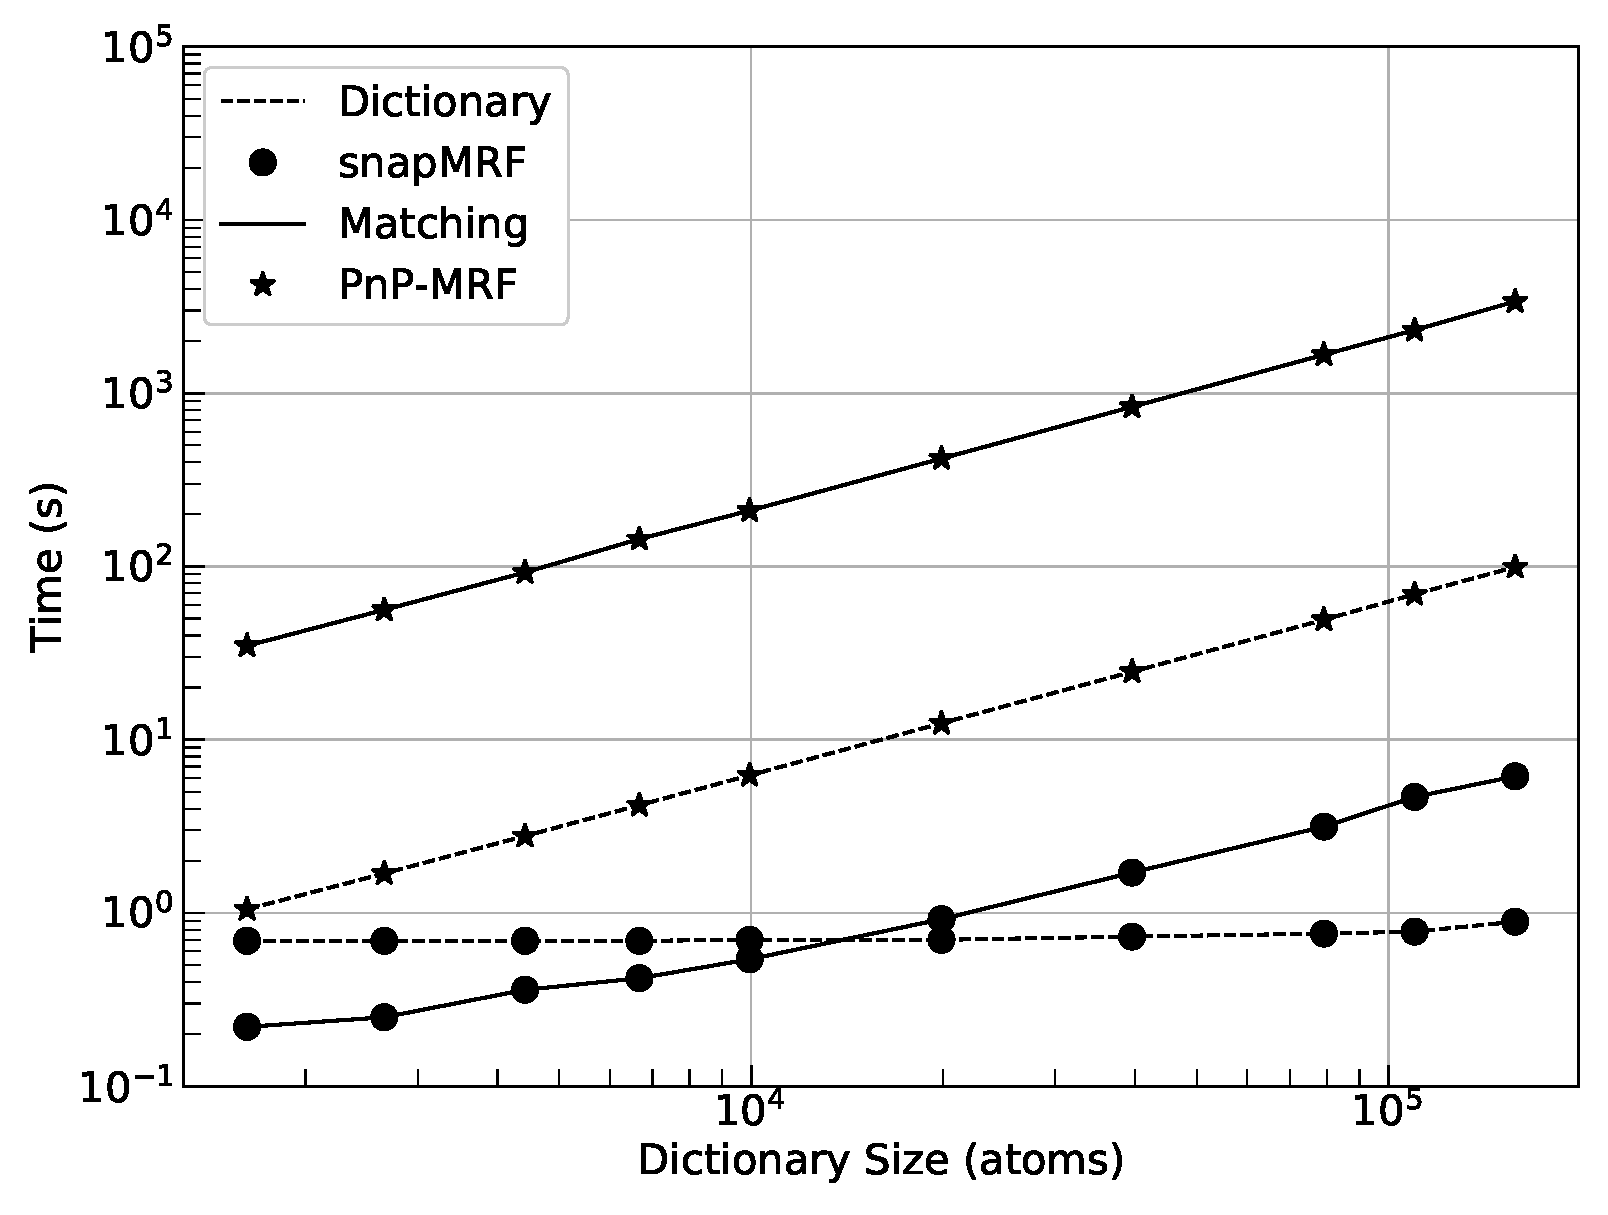
\includegraphics[width=0.8\textwidth]{img/snapmrf/time_vs_pnp.eps}
\end{subfigure}
\caption{字典生成和模板匹配运行时间比较。(上)snapMRF与EPG-X;(下)snapMRF与PnP-MRF。注意曲线为对数尺度。运行时间随着字典大小线性变化,说明了有效的并行化。在我们的例子中,对于240$\times$240个体素的指纹数据,模板匹配的时间比字典生成少得多。}
\label{fig:time}
\end{figure}

\subsection{体模数据的重建参数图}
snapMRF和EPG-X字典生成和模板匹配的运行时间在表\ref{tab:time}中。可以看出,对于不同的序列,snapMRF可以在15 s内生成大小为100,000的字典并进行模板匹配,速度远远大于EPG-X。

\begin{table}
\caption{snapMRF与EPG-X在字典生成和模板匹配上运行时间的比较}
\centering
\label{tab:time}
\begin{tabular}{|l|l|l|l|l|l|}
\hline
\hline
运行时间 & EPG-X & snapMRF & snapMRF & snapMRF\\ 
(s) & 固定$T_\mathrm{R}$ & 固定$T_\mathrm{R}$ & 变化$T_\mathrm{R}$ & 变化$T_\mathrm{R}$+$B_1^+$\\
\hline
体模/字典生成 & 17797.05 & 11.00 & 7.42 & 9.39 \\
\hline
体模/模板匹配 & 137.13 & 5.97 & 4.14 & 4.88\\
\hline
脑部/字典生成 & 18629.82 & 11.29 & 7.63 & 8.72 \\
\hline
脑部/模板匹配 & 143.55 & 6.13 & 4.23 & 4.63 \\
\hline
\end{tabular}
\end{table}

表\ref{tab:t1}和表\ref{tab:t2}分别展示了snapMRF和EPG-X在体模数据重建生成的$T_1$和$T_2$与对应的相对误差。两个表中的第一列分别为$T_1$和$T_2$的真实值。从\ref{tab:t1}和表\ref{tab:t2}中可以看出,对于固定$T_\mathrm{R}$序列,snapMRF与EPG-X的精度是几乎一样的的。这是自然的,因为snapMRF与EPG-X都是用EPG模型生成字典,重建的方法也都使用了模板匹配。对于变化$T_\mathrm{R}$序列,$T_1$的误差从5.0\%降低到了2.6\%,而$T_2$的误差保持不变。当我们考虑$B_1^+$的影响时,$T_1$的误差保持很低,$T_2$的误差降低到9.3\%。结果表明变化$T_\mathrm{R}$序列和$B_1^+$校正有助于提高参数图的准确性。

\begin{table}
\caption{snapMRF与EPG-X在体模数据上MRF生成$T_1$参数图的准确性比较。表中的第一列为$T_1$的真实值。snapMRF可以生成相当精确的$T_1$值,即使用了未经优化的序列和字典。}
\centering
\label{tab:t1}
\begin{tabular}{|l|l|l|l|l|l|}
\hline
\hline
真实$T_1$ & EPG-X & snapMRF & snapMRF & snapMRF\\ 
(ms) & 固定$T_\mathrm{R}$ & 固定$T_\mathrm{R}$ & 变化$T_\mathrm{R}$ & 变化$T_\mathrm{R}$+$B_1^+$\\
\hline
90.9 & 128.5 & 127.7 & 111.5 & 94.2\\
\hline
126.9 & 155.0 & 155.0 & 146.5 & 127.9\\
\hline
176.6 & 173.1 & 173.1 & 172.3 & 153.8\\
\hline
244.2 & 280.4 & 280.4 & 265.0 & 225.0\\
\hline
336.5 & 342.7 & 342.7 & 326.5 & 319.2\\
\hline
458.4 & 471.2 & 471.2 & 471.9 & 468.3\\
\hline
608.6 & 602.7 & 601.2 & 625.0 & 622.1\\
\hline
801.7 & 771.5 & 770.4 & 818.5 & 813.5\\
\hline
1044.0 & 945.0 & 943.1 & 1032.3 & 1026.0\\
\hline
1332.0 & 1262.7 & 1263.1 & 1310.8 & 1306.7\\
\hline
1604.0 & 1568.8 & 1568.1 & 1607.3 & 1593.3\\
\hline
1907.0 & 1861.2 & 1861.9 & 1854.2 & 1828.8\\
\hline
2173.0 & 2043.1 & 2043.1 & 2091.9 & 2094.2\\
\hline
2480.0 & 2366.5 & 2366.2 & 2434.6 & 2416.3\\
\hline
err (\%) & 4.9 & 5.0 & 2.6 & 3.0\\
 
\hline
\end{tabular}
\end{table}

\begin{table}
\caption{snapMRF与EPG-X在体模数据上MRF生成$T_2$参数图的准确性比较。表中的第一列为$T_2$的真实值。snapMRF可以生成相当精确的$T_2$值,即使用了未经优化的序列和字典。}
\centering
\label{tab:t2}
\begin{tabular}{|l|l|l|l|l|l|}
\hline
\hline
真实$T_2$ & EPG-X & snapMRF & snapMRF & snapMRF\\ 
(ms) & 固定$T_\mathrm{R}$ & 固定$T_\mathrm{R}$ & 变化$T_\mathrm{R}$ & 变化$T_\mathrm{R}$+$B_1^+$\\
\hline
5.6 & 6.9 & 6.9 & 9.4 & 12.3\\
\hline
7.9 & 11.5 & 11.2 & 10.0 & 13.5\\
\hline
11.2 & 13.3 & 13.3 & 11.2 & 13.5\\
\hline
15.8 & 13.7 & 13.5 & 11.3 & 20.4\\
\hline
22.6 & 21.2 & 21.2 & 23.3 & 30.0\\
\hline
32.0 & 32.3 & 32.3 & 38.3 & 47.3\\
\hline
46.4 & 45.0 & 44.8 & 50.4 & 60.0\\
\hline
64.1 & 64.2 & 64.2 & 70.2 & 83.8\\
\hline
96.9 & 84.6 & 84.4 & 90.8 & 104.6\\
\hline
133.3 & 144.0 & 143.8 & 146.9 & 170.8\\
\hline
190.9 & 175.4 & 175.4 & 185.2 & 213.8\\
\hline
278.1 & 266.5 & 266.5 & 255.4 & 290.0\\
\hline
403.5 & 323.3 & 323.5 & 343.7 & 407.7\\
\hline
581.3 & 474.0 & 474.2 & 453.5 & 531.5\\
\hline
err (\%) & 16.9 & 16.9 & 17.9 & 9.3\\

\hline
\end{tabular}
\end{table}

图\ref{fig:phantom}显示了snapMRF和EPG-X生成的$T_1$,$T_2$和质子密度参数图。为了更好地观察感兴趣区域,我们用Otsu方法从质子密度图像中生成了一个掩膜,并应用到$T_1$和$T_2$参数图中。这样做可以去除背景中的高信号(研究对象之间用于填充的水),使得感兴趣区域凸现出来。另外,我们也简单地去除了外围的伪影。在绘制参数图时,$T_1$图显示在0--2500 ms的范围,$T_2$图显示在0--800 ms范围。从图\ref{fig:phantom}中可以看出,对于固定$T_\mathrm{R}$序列,snapMRF和EPG-X所生成的参数图在视觉上几乎一致。对于变化$T_\mathrm{R}$序列,$T_1$参数图有所提高,而$T_2$参数图保持不变。当考虑$B_1^+$校正时,$T_2$参数图也有了明显的提升。

\begin{figure}[htbp]
\centerline{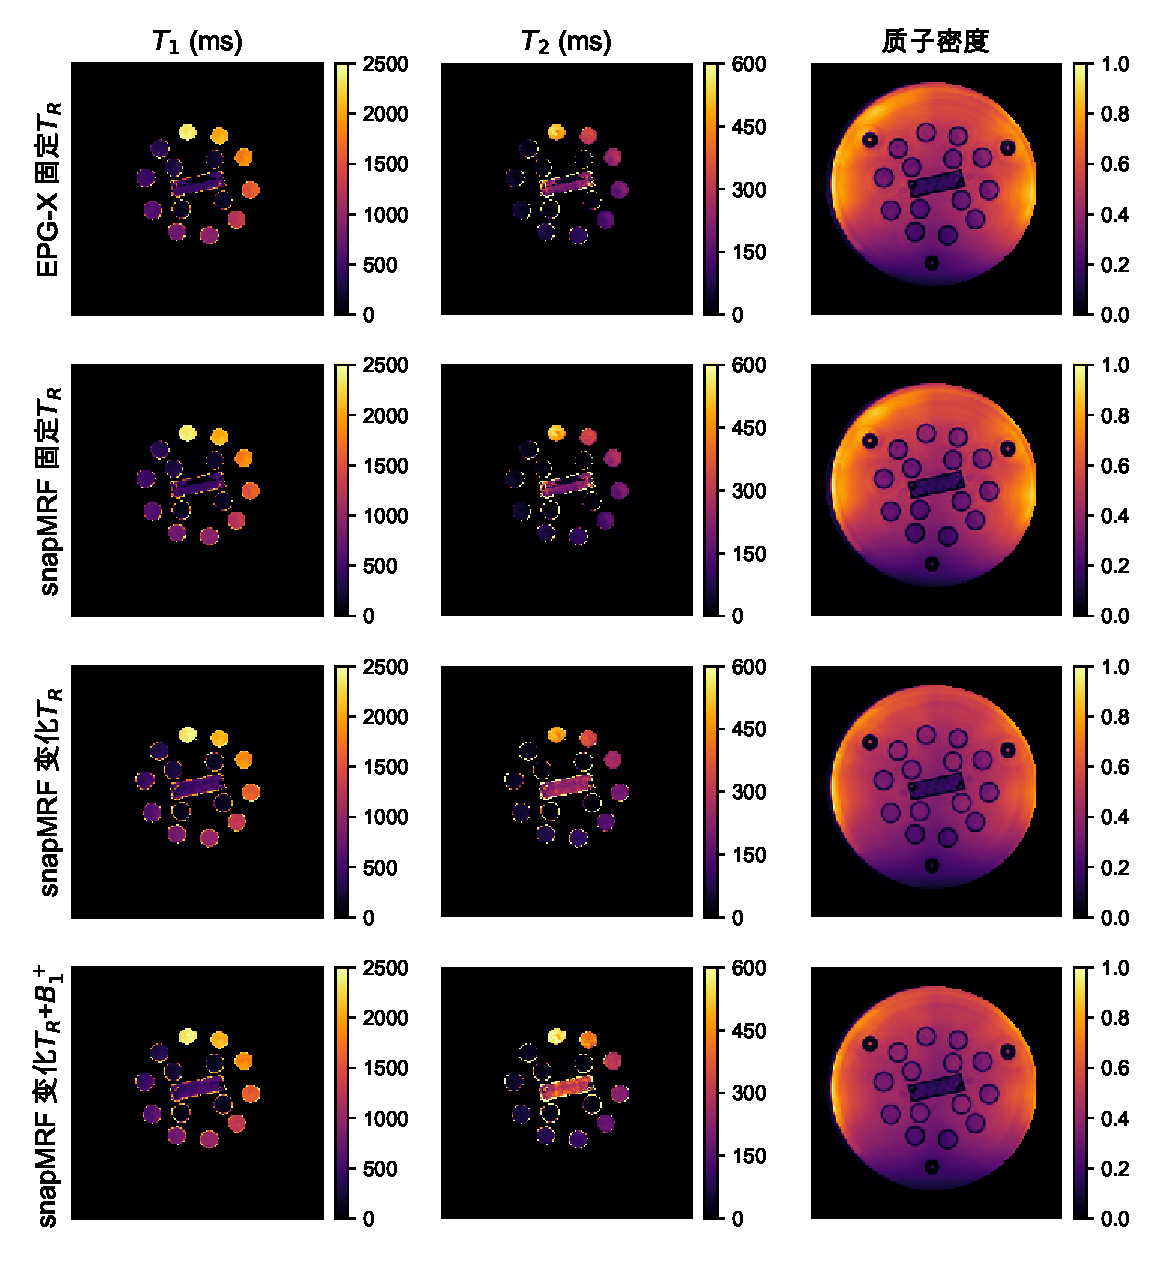
\includegraphics[width=1\textwidth]{img/snapmrf/figure2.eps}}
\caption{snapMRF和EPG-X在体模数据上参数准确度的比较。第一行:EGP-X使用固定$T_\mathrm{R}$生成的参数图。从左到右分别为$T_1$,$T_2$和质子密度。第二行到第四行为snapMRF的重建结果,使用的序列分别为固定$T_\mathrm{R}$、变化$T_\mathrm{R}$和考虑$B_1^+$的变化$T_\mathrm{R}$。$T_1$和$T_2$的定量估计在\ref{tab:t1}和表\ref{tab:t2}中。运行时间显示在表\ref{tab:time}中。在所有的$T_1$和$T_2$参数图中,为了更好的视觉效果,用于填充体模的背景中的水信号被人为的抑制。
}
\label{fig:phantom}
\end{figure}

\subsection{活体人脑数据的重建参数图}
图\ref{fig:brain}显示了snapMRF在活体人脑数据中的表现以检测snapMRF是否可以生成干净的活体参数图。为了更好地视觉效果,与体模数据相同,我们使用Otsu方法生成了一个掩膜,并将其作用在$T_1$和$T_2$参数图上。在绘制参数图时,$T_2$参数图显示在0--300 ms的范围,质子密度图像显示在0--0.25的范围。程序运行时间在表\ref{tab:time}中。

\begin{figure}[htbp]
\centerline{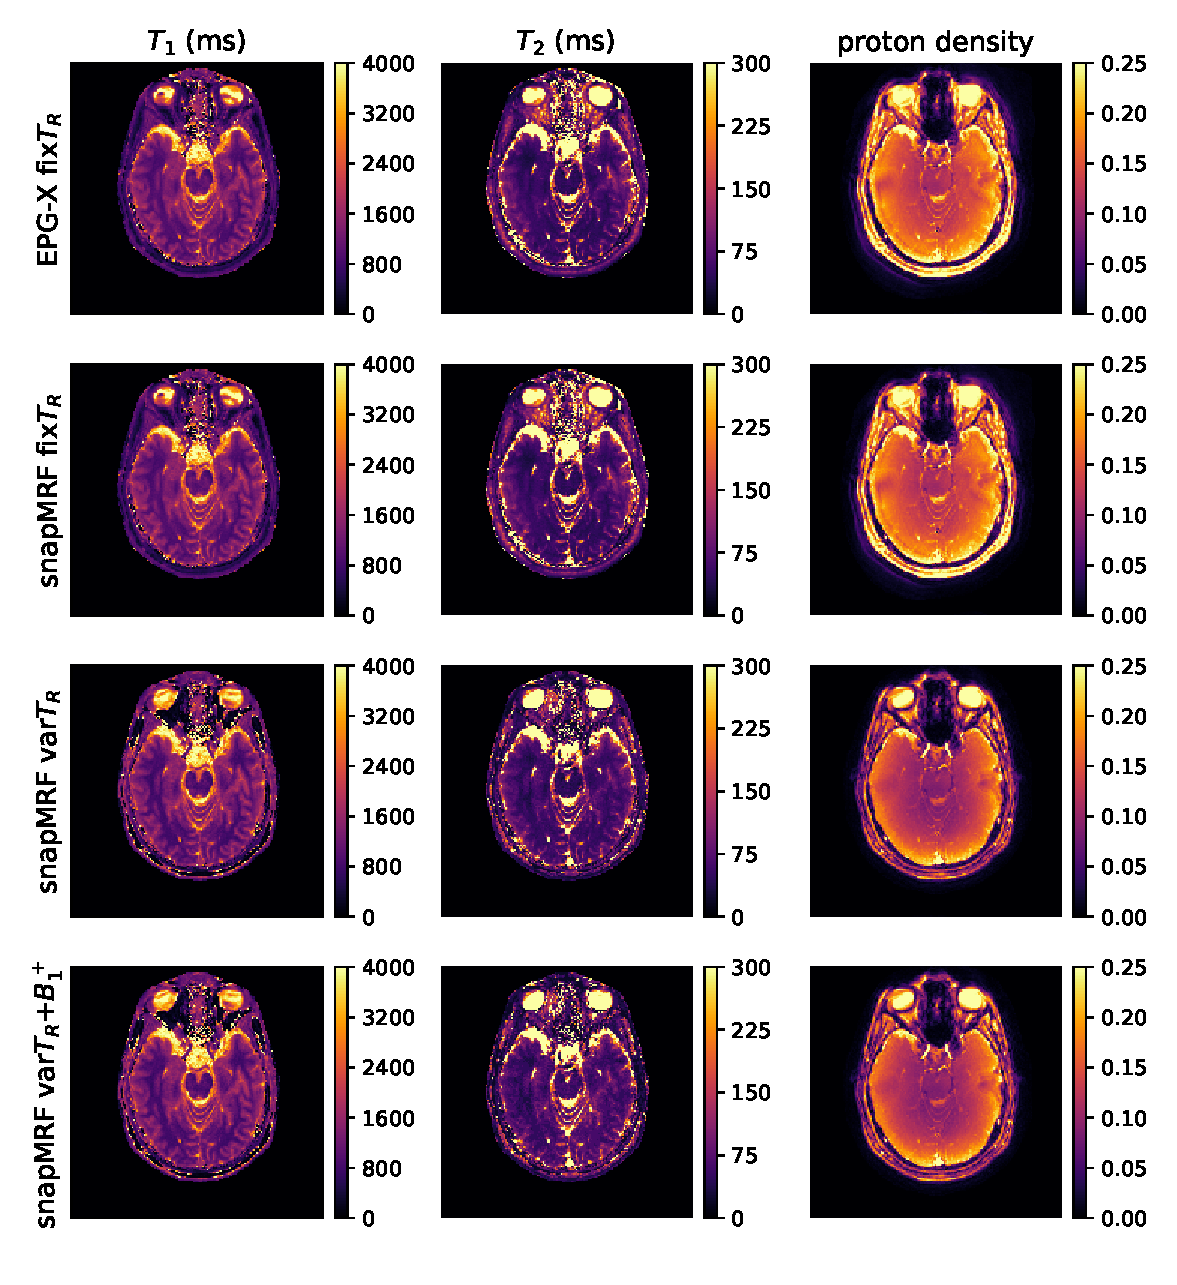
\includegraphics[width=1\textwidth]{img/snapmrf/figure3.eps}}
\caption{snapMRF和EPG-X在活体人脑数据上参数准确度的比较。第一行:EGP-X使用固定$T_\mathrm{R}$生成的参数图。从左到右分别为$T_1$,$T_2$和质子密度。第二行到第四行为snapMRF的重建结果,使用的序列分别为固定$T_\mathrm{R}$、变化$T_\mathrm{R}$和考虑$B_1^+$的变化$T_\mathrm{R}$。运行时间显示在表\ref{tab:time}中。所有的序列下,snapMRF都可以得到质量较好的图像。}
\label{fig:brain}
\end{figure}

从图\ref{fig:brain}中可以看出,对于所有序列,snapMRF都可以生成高质量的参数图。与体模数据的情况类似,snapMRF和EPG-X在固定$T_\mathrm{R}$序列时生成了视觉上一致的参数图。对于变化$T_\mathrm{R}$序列,$T_1$参数图更加平滑并且质子密度参数图也比固定$T_\mathrm{R}$时更暗一些。当考虑$B_1^+$时校正时,$T_2$参数图也变得更平滑,尤其是在灰质区域。

\section{数值实验分析}
在本文中,我们基于MRF字典生成与模板匹配运行时间慢的缺点,推出了一款新的基于GPU的程序snapMRF,用于MRF字典生成与模板匹配。snapMRF可以快速并准确地生成参数图,当字典较小时,可以达到实时效果。与其他开源的程序相比,字典生成的速度提高了100--1000倍,模板匹配的速度提高了10--100倍。snapMRF的另一个优势是它适用于不同类型的MRF序列,包括在MRF中经常使用的变化$T_\mathrm{R}$序列与$B_1^+$校正。

snapMRF可以达到神经网络的推断速度,并且运行时间与序列的选择无关。而且,如果研究人员仍然希望通过训练神经网络来进行参数图的重建,snapMRF可以用来进行训练集,即字典的生成。另外,snapMRF的快速度可以用来减少多个经历不同$B_1^+$振幅的位置的计算时间。这适用于图像射频场的变化,也适用于切片轮廓\cite{Ma_B1_MRF}的变化。

snapMRF中选择了EPG模型来进行字典的生成,主要原因除了EPG可以表征失相场这个特征之外,EPG模型可以比较方便的加入其它因素的影响,比如化学位移(chemical shift)、磁化转移(magnetization transfer)\cite{Hamilton}、运动、扩散等。目前snapMRF可以实现的使用变化$T_\mathrm{R}$序列对$B_1^+$效应进行建模。之后我们会把前面提到因素加入到snapMRF中。

snapMRF全部在单一GPU上运行,但是snapMRF在未来也可以被设置为在多个GPU上运行,如文献\cite{tron}中所用。理论上来说,snapMRF的加速率会和GPU的个数成正比,因为在snapMRF中字典生成的并行计算是关于每个字典元素的,而模板匹配是关于每个指纹体素的。

\section{本章小结}
在本章中,我们首先介绍了磁共振指纹研究的背景意义和所存在的问题。针对MRF中字典生成与模板匹配速度慢的问题,我们开发了一款基于GPU的程序snapMRF。我们给出了snapMRF的编程思路和主要流程,并简单介绍了核函数。我们将snapMRF与开源程序EPG-X和PnP-MRF进行了比较。运行时间上,snapMRF整体提高了MRF生成参数图的速度,其中字典生成的速度提高了100--1000倍,模板匹配的速度提高了10--100倍。参数图精度上,由于可以处理多种MRF序列,snapMRF可以生成更加精确地参数图。未来我们会在snapMRF中加入更多的功能,如切片轮廓等。





















